\documentclass[13pt]{beamer}
\usetheme{Frankfurt}
\usecolortheme{beaver}
\graphicspath{ {img/} }


\usepackage[spanish]{babel}
\usepackage{amsmath}
\usepackage{amsfonts}
\usepackage{amssymb}
\usepackage{color}
\usepackage{xcolor}
\usepackage{listings}
\usepackage{graphicx}
\usepackage{wrapfig}
\usepackage{algorithm2e}

\RestyleAlgo{ruled}
\SetKwComment{Comment}{/* }{ */}

\makeatletter
\renewcommand{\algorithmcfname}{Algoritmo}
\makeatother

\SetKwFor{While}{mientras }{}{fin}
\SetKwFor{For}{para cada }{}{fin}
\SetKwFor{If}{si}{}{fin}
%\SetKwFor{eIf}{si}{}{en otro caso}
% \SetKwFor{For}{para cada:}{}{}
%\SetKwFor{KwData}{Dato:}{}{}
%\SetKwFor{Data}{Dato:}{}{}
\SetKwFor{Results}{resultado}{}{}


\definecolor{codegreen}{rgb}{0,0.6,0}
\definecolor{codegray}{rgb}{0.5,0.5,0.5}
\definecolor{codepurple}{rgb}{0.58,0,0.82}
\definecolor{backcolour}{rgb}{0.95,0.95,0.92}

\lstdefinestyle{mystyle}{
    basicstyle=\tiny,
    commentstyle=\color{codegreen},
    keywordstyle=\color{magenta},
    numberstyle=\tiny\color{codegray},
    stringstyle=\color{codepurple},
    basicstyle=\ttfamily\footnotesize,
    breakatwhitespace=false,         
    breaklines=true,                 
    captionpos=b,                    
    keepspaces=true,                 
    numbers=left,                    
    numbersep=5pt,                  
    showspaces=false,                
    showstringspaces=false,
    showtabs=false,                  
    tabsize=2,
	xleftmargin=8pt
}

\lstset{literate=
	{á}{{\'a}}1 {é}{{\'e}}1 {í}{{\'i}}1 {ó}{{\'o}}1 {ú}{{\'u}}1
	{Á}{{\'A}}1 {É}{{\'E}}1 {Í}{{\'I}}1 {Ó}{{\'O}}1 {Ú}{{\'U}}1
	{à}{{\`a}}1 {è}{{\`e}}1 {ì}{{\`i}}1 {ò}{{\`o}}1 {ù}{{\`u}}1
	{À}{{\`A}}1 {È}{{\'E}}1 {Ì}{{\`I}}1 {Ò}{{\`O}}1 {Ù}{{\`U}}1
	{ä}{{\"a}}1 {ë}{{\"e}}1 {ï}{{\"i}}1 {ö}{{\"o}}1 {ü}{{\"u}}1
	{Ä}{{\"A}}1 {Ë}{{\"E}}1 {Ï}{{\"I}}1 {Ö}{{\"O}}1 {Ü}{{\"U}}1
	{â}{{\^a}}1 {ê}{{\^e}}1 {î}{{\^i}}1 {ô}{{\^o}}1 {û}{{\^u}}1
	{Â}{{\^A}}1 {Ê}{{\^E}}1 {Î}{{\^I}}1 {Ô}{{\^O}}1 {Û}{{\^U}}1
	{ã}{{\~a}}1 {ẽ}{{\~e}}1 {ĩ}{{\~i}}1 {õ}{{\~o}}1 {ũ}{{\~u}}1
	{Ã}{{\~A}}1 {Ẽ}{{\~E}}1 {Ĩ}{{\~I}}1 {Õ}{{\~O}}1 {Ũ}{{\~U}}1
	{œ}{{\oe}}1 {Œ}{{\OE}}1 {æ}{{\ae}}1 {Æ}{{\AE}}1 {ß}{{\ss}}1
	{ű}{{\H{u}}}1 {Ű}{{\H{U}}}1 {ő}{{\H{o}}}1 {Ő}{{\H{O}}}1
	{ç}{{\c c}}1 {Ç}{{\c C}}1 {ø}{{\o}}1 {å}{{\r a}}1 {Å}{{\r A}}1
	{€}{{\euro}}1 {£}{{\pounds}}1 {«}{{\guillemotleft}}1
	{»}{{\guillemotright}}1 {ñ}{{\~n}}1 {Ñ}{{\~N}}1 {¿}{{?`}}1 {¡}{{!`}}1 
}

\lstset{style=mystyle, basicstyle=\scriptsize}

\author{Shao Jie Hu Chen \and Mario Megías Mateo \and Jesús Samuel García Carballo}
\title{Práctica 4. Programación Dinámica}
\subtitle{Algorítmica}
%\logo{
\includegraphics[scale=0.05]{logo-ugr.jpeg}}
\institute{Equipo Rojo}
%\date{}
%\subject{}
%\setbeamercovered{transparent}
\setbeamertemplate{navigation symbols}{}

\begin{document}
	
	\begin{frame}[plain]
		\maketitle
		% \begin{center}
		% 	
\includegraphics[scale=0.15]{logo-ugr.jpeg}
		% \end{center}
	\end{frame}
	
	\begin{frame}
		\frametitle{Índice de contenidos}
		\tableofcontents
	\end{frame}

    % Introducción

    \section{Introducción}

	\begin{frame}
		\frametitle{Objetivos}
        \begin{itemize}
            \item Conocer qué es la programación dinámica.
            \item Saber determinar si un algoritmo es de programación dinámica.
            \item Ser capaces de implementar un algoritmo de programación dinámica.
        \end{itemize}
	\end{frame}

	\begin{frame}
		\frametitle{Programación Dinámica}
        La programación dinámica es un método de diseño de algoritmos que se puede usar cuando la solución del 
        problema se puede ver como el resultado de una sucesión de decisiones. 
        Proporciona un procedimiento sistemático para encontrar la combinación de decisiones que maximice la efectividad
        total, al descomponer el problema en etapas, todas ellas enlazadas mediante algoritmos recursivos.
	\end{frame}

    \begin{frame}
		\frametitle{Origen}
            \begin{figure}[H] 
                \centering
                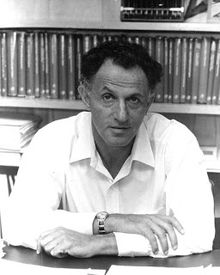
\includegraphics[width=0.5\textwidth]{bellman.jpg}
                \caption{Richard Bellman}
            \end{figure}
    \end{frame}

	\begin{frame}
		\frametitle{Características}
        En líneas generales un algoritmo de Programación Dinámica se aplica en cuatro fases:
        \begin{itemize}
        \item Naturaleza n-etápica del problema.
        \item Verificación del Problema de Optimalidad.
        \item Planteamiento de una recurrencia.
        \item Cálculo de la solución(enfoque adelantado o retardado). 
        \end{itemize}
	\end{frame}

	\section{Comparación de ADN}

    \begin{frame}
        \frametitle{Enunciado}
        Dos hermanos fueron separados al nacer y mediante un programa de televisión se han
        enterado que podrían ser hermanos. Ante esto, los dos están de acuerdo en hacerse un test de
        ADN para verificar si realmente son hermanos. Se debe encontrar el porcentaje de similitud que existe 
        entre estos posibles hermanos, $($como es un ejemplo lo haremos para 2 entradas posibles$)$.
    \end{frame}

    \begin{frame}
        \frametitle{Metodología}
        \begin{figure}[H] 
            \centering
            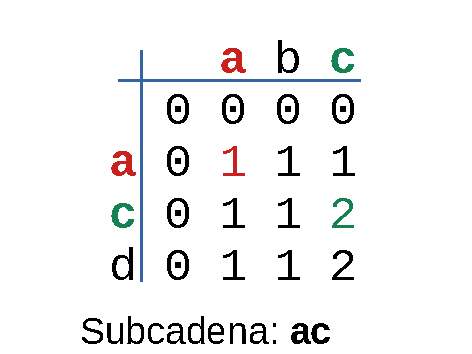
\includegraphics[width=0.85\textwidth]{dibujito.pdf}
        \end{figure}
    \end{frame}



    \begin{frame}
        \frametitle{Pseudocódigo}
        \begin{algorithm}[H]
            \caption{Algoritmo para la matriz que calcula la subsecuencia con mayor similitud.}\label{alg:simil}
            \begin{minipage}{0.92\textwidth}
            \textbf{Parámetro}: string (palabra1)\;
            \textbf{Parámetro}: string (palabra2)
            \end{minipage}
          
            int matriz[MAX][MAX] = {0}\;
            int longitud=0\;
            string subsecuencia\;
          
            \For{i desde 1 $\leq$ palabra1.size y ++i} {
              \For{j desde 1 $\leq$ palabra2.size y ++j} {
                \eIf{palabra1[i-1] == palabra2[j-1]}{
                  matriz[i][j] = matriz[i-1][j-1]+1\;
                }{ matriz[i][j] = max(matriz[i][j-1],matriz[i-1][j])\;}
              }
            }
          \end{algorithm}
    \end{frame}

	\begin{frame}
		\frametitle{Análisis de eficiencia}
		
		\begin{block}{Eficiencia teórica}
			\centering
			$O(n^{2})$
		\end{block}
		
	\end{frame}

    \begin{frame}
		\frametitle{Aplicabilidad de la programación dinámica}
        \begin{enumerate}
            \item Comprobación de la naturaleza n-etápica del problema. 
            \item Verificación del principio de optimalidad de Bellman. 
            \item Construcción de una ecuación recurrente. 
            \item Cálculo de la solución(enfoque adelantado o retardado). 
        \end{enumerate}
	\end{frame}

    \begin{frame}
		\frametitle{Comprobación de la naturaleza n-etápica del problema}
        En efecto, como primera etapa se ha de conseguir las subsecuencias más largas de longitud 1, 
        después obtener las subsecuencias más largas de longitud 2 y, así, sucesivamente. 
	\end{frame}

    \begin{frame}
		\frametitle{Verificación del principio de optimalidad de Bellman}

        \begin{alertblock}{Teorema de optimalidad}
            Sean $X=(x_1,x_2,\cdots, x_m),Y=(y_1,y_2, \cdots, y_n)$ secuencias de caracteres 
            y sea $Z$ cualquier subsecuencia común máxima 
            de $X$ e $Y$. Entonces:
            \begin{enumerate}
              \item Si $x_m = y_n$, entonces $z_k = x_m = y_n$ y $Z_{k-1}$ es una subsecuencia
              común máxima de $X_{m-1}$ e $Y_{n-1}$. 
              \item Si $x_m \neq y_n$, entonces:
              \begin{enumerate}
                \item $z_k \neq x_m$ implica que $Z$ es una subsecuencia común máxima para $X_{m-1}$ e $Y$. 
                \item $z_k \neq y_n$ implica que $Z$ es una subsecuencia común máxima para $X$ e $Y_{n-1}$. 
              \end{enumerate}
            \end{enumerate}
        \end{alertblock}
	\end{frame}

    \begin{frame}
		\frametitle{Construcción de una ecuación recurrente}
        Sean $n,m \in \mathbb{N}$, dadas dos secuencias $X = { x_1,x_2,...,x_m}$ e $Y = { y_1,y_2,...,y_n}$, llamaremos $L(i,j)$ a la 
        longitud de la secuencia común máxima de las secuencias $X_i = {x_1,...,x_i}$ e $Y_j = {y_1,...,y_j}$ $\forall i \in {1,...,n} $ y $\forall i \in {1,...,m}$, 
        que se define como:  

        \[
        L(i,j) = 
        \left \{
            \begin{aligned}
            0 &,\ \text{si} \ i = 0 \ o \ j = 0\\
            L(i,j) + 1 &,\ \text{si} \ i \neq  1 , j \neq  0 \ y \ x_i = y_j\\
            max(L(i,j-1) , L(i-1,j))&,\ \text{si} \ i \neq 1 , j \neq 0 \ y \ x_i \neq y_j
            \end{aligned}
        \right .
        \]
	\end{frame}



    \begin{frame}
		\frametitle{Cálculo de la solución}
        \begin{figure}
            \centering
            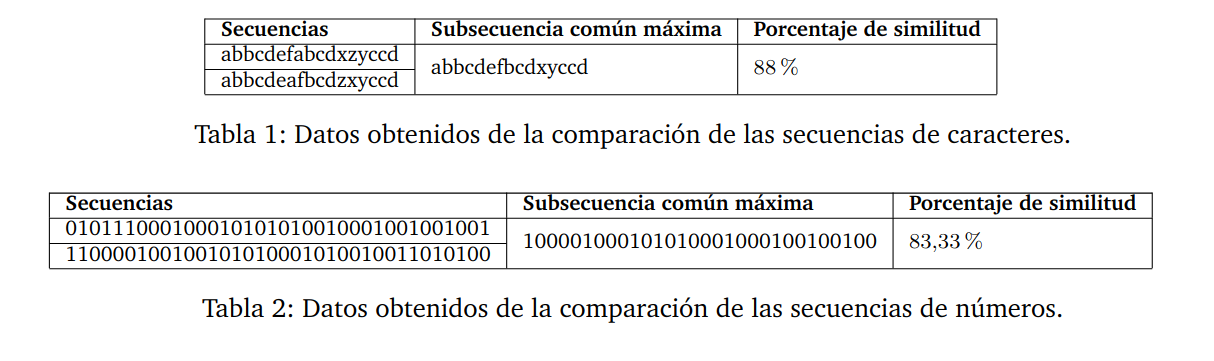
\includegraphics[width=10cm, height=5cm]{table.png}
          \end{figure}
	\end{frame}


    \begin{frame}
		\frametitle{Resultado}
        \begin{figure}
            \centering
            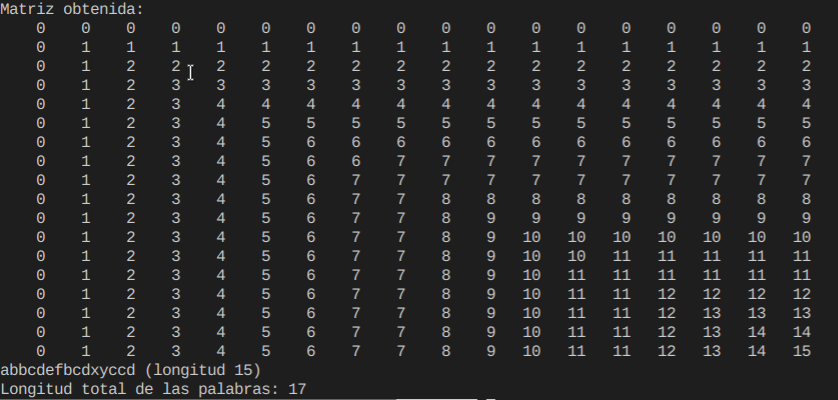
\includegraphics[scale=0.55]{LettersMatrixResult.png}
          \end{figure}
	\end{frame}
	
	\section{Comparativa con fuerza bruta}
	
	\begin{frame}
		\frametitle{Fuerza bruta}
		\begin{figure}
			Calculamos todas las subcadenas de cada cadena y nos quedamos con la
			común de mayor longitud.
			
			\begin{block}{Eficiencia teórica}
				\centering
				$O(2^{n})$
			\end{block}
			
		\end{figure}
	\end{frame}

    \begin{frame}
		\frametitle{Comparación de tiempos}
		\begin{figure}[h]
            \centering
            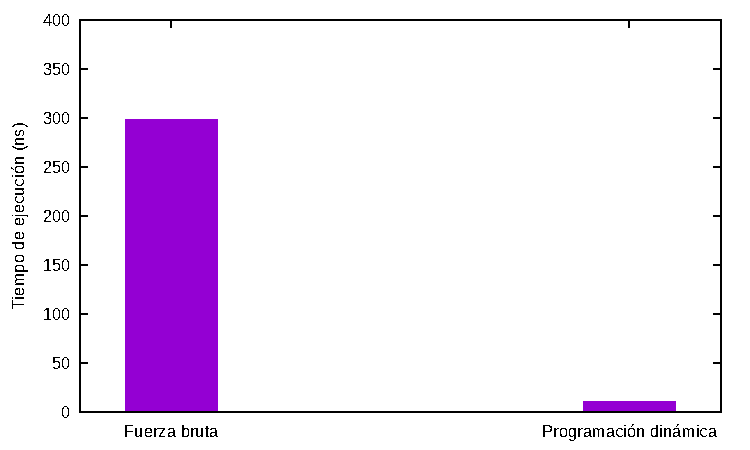
\includegraphics[scale=0.7]{comparativa.pdf}
            \caption{Gráfica con los tiempos de ejecución (en $\mu s$) en la ejecución de los algoritmos de fuerza bruta
            y dinámicos para $n=5$. }
            \label{graph:comp}
          \end{figure}
	\end{frame}
	
	\section{Conclusion}

    \begin{frame}
		\frametitle{Conclusion}
        \begin{itemize}
            
            \item Existen problemas cuya resolución por medio de algoritmos de fuerza 
            bruta presentan una complejidad no polinomial, sin embargo con el uso de la 
            técnica de programación dinámica \textbf{podemos reducir la eficiencia a un orden 
            polinomial}. En nuestro ejemplo, \textbf{pasamos de un orden de eficiencia exponencial
            a un orden polinómico}, lo cual \textbf{supone una enorme mejora en cuanto al tiempo de 
            ejecución}.
            
            \item La técnica de programación dinámica proporciona algoritmos con órdenes de eficiencia
            polinomiales, pero esta mejora en tiempo de ejecución supone una \textbf{mayor sobrecarga en cuanto 
            a los recursos de memoria consumidos}. En nuestro ejemplo, el problema trabaja sobre dos cadenas de
            $n$ componentes, pero para la realización del algoritmo \textbf{necesitamos construir una matriz de $n^{2}$ 
            entradas, aumentando considerablemente el uso de la memoria del computador}.

            \item Además de la mejora en eficiencia respecto de algoritmos triviales, la técnica de programación
            dinámica se destaca por la \textbf{obtención de soluciones óptimas respecto a la toma de la primera decisión}.
            
            
        \end{itemize}
	\end{frame}

    % Bibliografía

    \section{Bibliografía}

    \begin{frame}
        \begin{thebibliography}{0}
            \bibitem{Verdegay2017} Verdegay Galdeano. (2017). Lecciones de Algorítmica / José Luis Verdegay. Técnica Avicam.
            \bibitem{Cormen2017} Cormen. (2017). Introduction to algorithms / Thomas H. Cormen... [et al.] (3rd ed.). PHI Learning.
            \bibitem{Garrido2018} Garrido Carrillo. (2018). Estructuras de datos avanzadas: con soluciones en C++ / A. Garrido. Universidad de Granada.  
        \end{thebibliography}
    \end{frame}

\end{document}
